% !TeX TS-program = lualatex
\documentclass[11pt,letterpaper]{article}
\usepackage{polyglossia} %configuracion de idioma
\setmainlanguage{spanish} %elegir idioma español
\usepackage{fontspec} %paquete para cargar fuentes
\setsansfont{cmunb}[Extension=.otf,
UprightFont=*mr,
ItalicFont=*mo,
BoldFont=*sr, % semibold
BoldItalicFont=*so, % semibold oblique
NFSSFamily=cmbr]
\usepackage{cmbright} %fuentes
\usepackage{microtype} %mejorar generales al documento pdf
\usepackage{amsmath} %paquete matematicos
\usepackage{amsfonts} %fuentes matematicas varias
\usepackage{amssymb} %simbolos matematicos varios
\usepackage{graphicx} %incluir graficos
\usepackage[left=2cm, right=2cm, top=2cm, bottom=2cm]{geometry} %paquete de configuracion de margenes
\usepackage[dvipsnames]{xcolor} %paquete de colores
\usepackage[backend=biber, style=apa]{biblatex} %Biblo APA
\DeclareLanguageMapping{spanish}{spanish-apa} %Idioma Apa
\addbibresource{Biblioteca.bib} %Archivo .bib
\setlength{\bibitemsep}{0.6\baselineskip}
\begin{document}
	\section{Introducción}
	
	El método más común para transportar fluidos de un punto a otro es impulsarlo a través de un sistema de tuberías. Las tuberías de sección circular son las más frecuentes, ya que esta forma ofrece no solo mayor resistencia estructural sino también mayor sección transversal para el mismo perímetro exterior que cualquier otra forma. \parencite[1.1]{crane}
	
	\section{Propiedades físicas de los fluidos}
	
	La solución de cualquier problema de flujo de fluidos requiere un conocimiento previo de las propiedades físicas del fluido en cuestión. A continuación se presentan algunas de ellas.
	
	\subsection{Viscosidad}
	
	La viscosidad expresa la facilidad que tiene un fluido para fluir cuando se le aplica una fuerza externa. La viscosidad absoluta de un fluido, es una medida de su resistencia al desplazamiento o  a sufrir deformaciones internas. \parencite[1.2]{crane}
	
	\subsection{Densidad}
	
	La densidad de una sustancia es su masa por unidad de volumen \parencite{crane}. En el estudio de los fluidos es conveniente suponer que los fluidos están continuamente distribuidos en toda una región de interés, es decir es tratado como un medio continuo. La principal propiedad que se usa para determinar si la suposición de medio continuo es apropiada es la densidad.\parencite[10]{merle}
	
	\section{Presión}
	
	El flujo de fluidos en tuberías está siempre acompañado de rozamiento de las partículas del fluido entre sí y, consecuentemente, por la pérdida de energía disponible, en otras palabras, tiene que existir una perdida de presión en el sentido del flujo. Si se conectaran dos manómetros a una tubería por la que pasa un fluido como en \ref{tuberia}, el manómetro $P_1$, indicara una presión estática mayor que el manómetro $P_2$ \parencite[1.7]{crane}
	
		\begin{figure}[H]
			\centering
			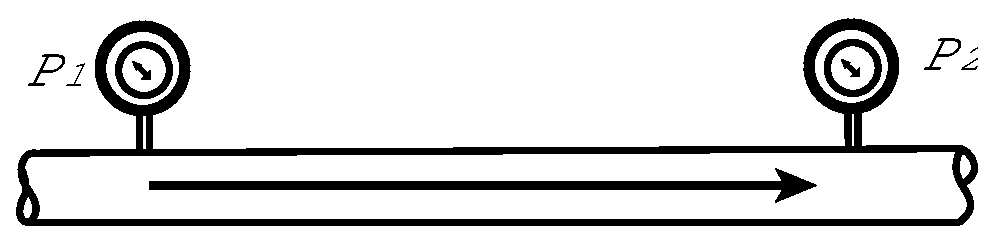
\includegraphics[width=0.6\linewidth]{Vectores/Tuberia_manometros}
			\caption{La flecha indica el sentido del flujo. Figura adaptada de \parencite[1.7]{crane}}
			\label{tuberia}
		\end{figure}
	
	\printbibliography[title={Referencias}]
	
\end{document}